\chapter[]{Appendix example}
\section{Dining Philosophers}\label{app:dining_phil}
The Dining Philosophers problem is defined as follows:
\bsqoute{Five philosophers spend their lives thinking and eating. The philosophers share a common dining room where there is a circular table surrounded by five chairs, each belonging to one philosopher. In the center of the table there is a large bowl of spaghetti, and the table is laid with five forks (see \bsref{fig:dining_philosophers}). On feeling hungry, a philosopher enters the dining room, sits in his own chair, and picks up the fork on the left of his place. Unfortunately, the spaghetti is so tangled that he needs to pick up and use the fork on his right as well. When he has finished, he puts down both forks, and leaves the room. The room should keep a count of the number of philosophers in it.}{Edgar Dijkstra\cite[p. 673]{hoare1978communicating}}

\begin{figure}[htbp]
\centering
 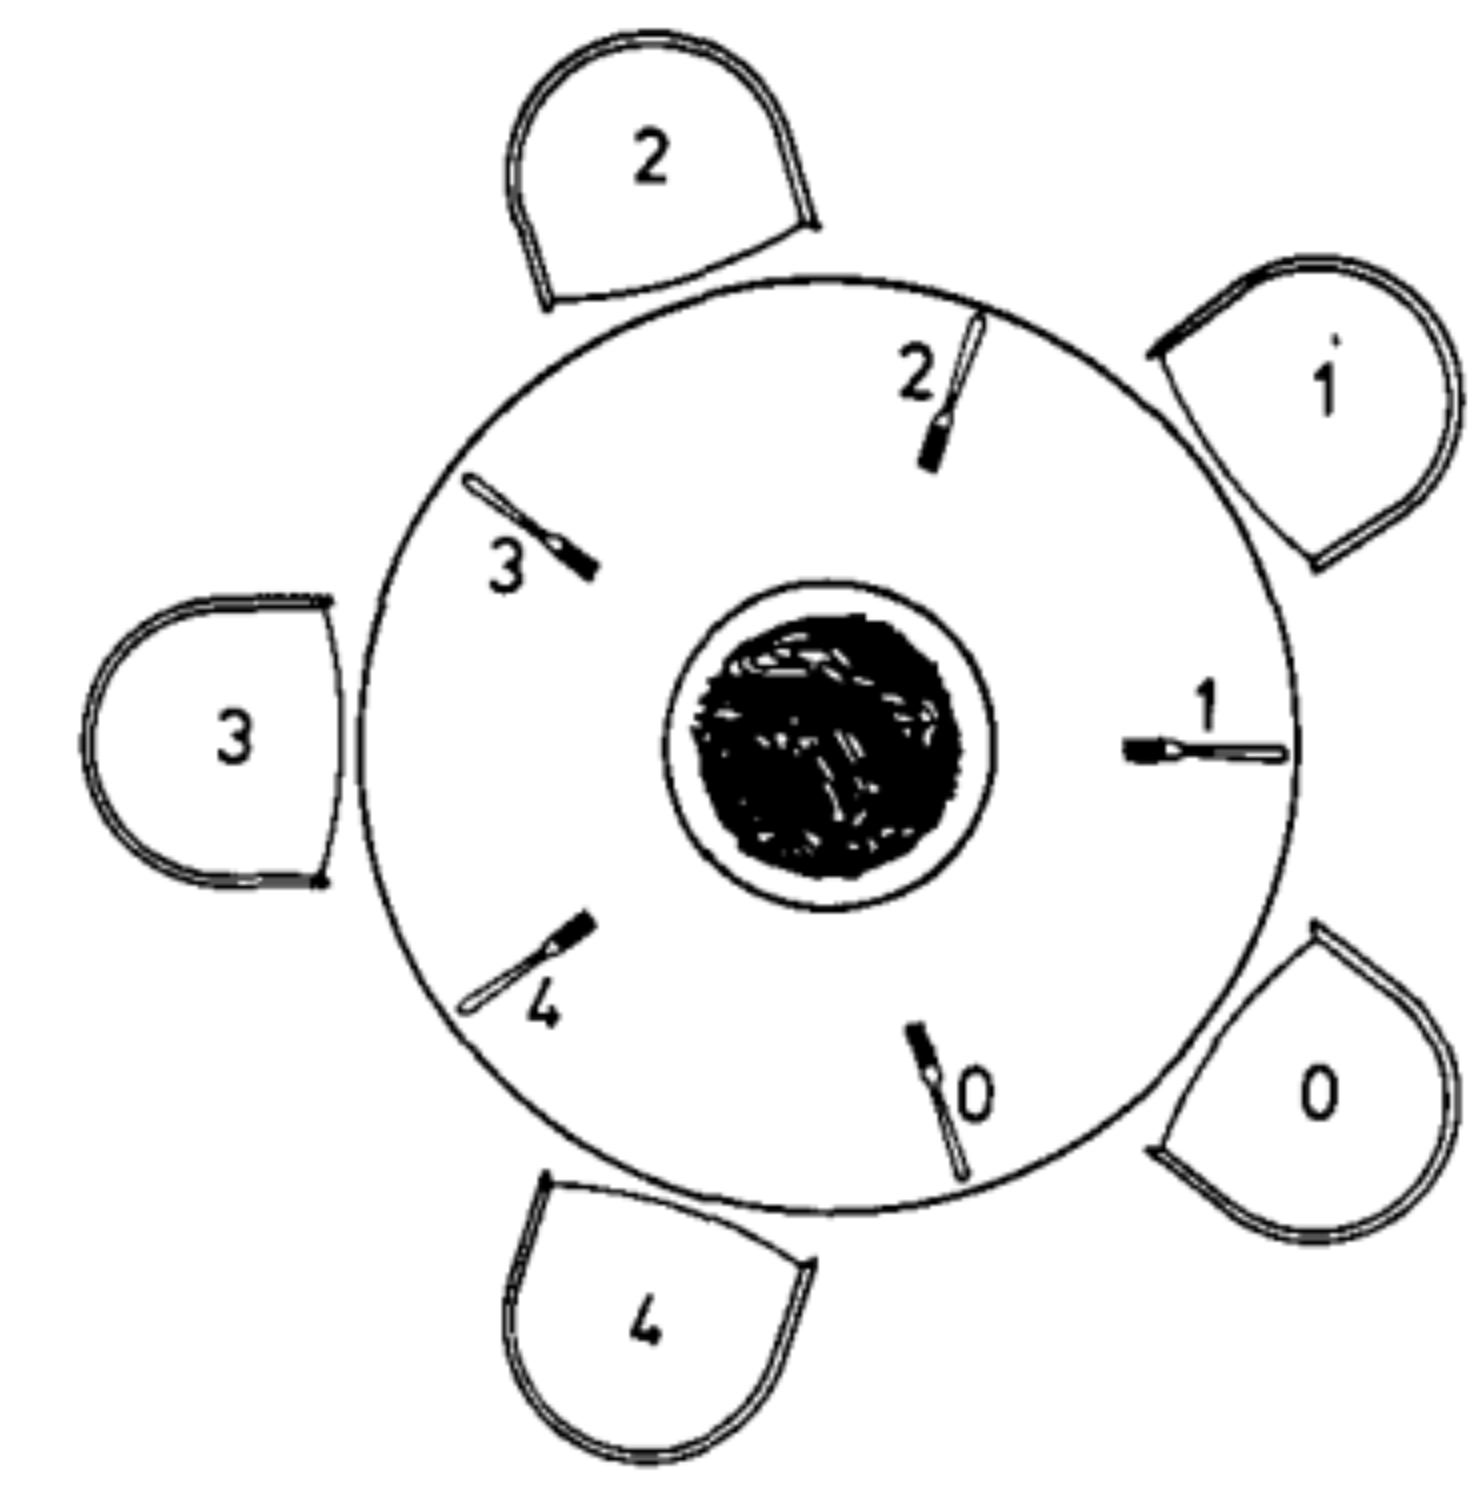
\includegraphics[width=0.7\textwidth]{\rootpath/worksheets/appendix/figures/dining_philosophers}
 \caption{The Dining Philosophers}
\label{fig:dining_philosophers}
\end{figure}

\section{The Santa Claus Problem}\label{app:santa}
The Santa Claus problem is defined as follows:
\bsqoute{Santa Claus sleeps in his shop up at the North Pole, and can only be wakened by either all nine reindeer being back from their year long vacation on the beaches of some tropical island in the South Pacific, or by some elves who are having some difficulties making the toys. One elf's problem is never serious enough to wake up Santa (otherwise, he may \b{never} get any sleep), so, the elves visit Santa in a group of three. When three elves are having their problems solved, any other elves wishing to visit Santa must wait for those elves to return. If Santa wakes up to find three elves waiting at his shop's door, along with the last reindeer having come back from the tropics, Santa has decided that the elves can wait until after Christmas, because it is more important to get his sleigh ready as soon as possible. (It is assumed that the reindeer don't want to leave the tropics, and therefore they stay there until the last possible moment. They might not even come back, but since Santa is footing the bill for their year in paradise … This could also explain the quickness in their delivering of presents, since the reindeer can't wait to get back to where it is warm.) The penalty for the last reindeer to arrive is that it must get Santa while the others wait in a warming hut before being harnessed to the sleigh.}{John A. Trono\cite{trono1994new}}

\section{Concurrent HashMap}\label{app:hashmap}
A HashMap is a data structure for implementing dictionary, that is a structure which allows looking up values based on a key. It provides the operations Insert, Search, and Delete. It is useful due to its property of giving an average time of O(1) for all operations under reasonable assumptions\cite[p. 253]{cormen2009introduction}. Implementation details of a HashMap may vary, but traditionally\andreas{Hmm. In java and c\#..?} follows the following concept\cite[p. 253]{cormen2009introduction}. Internally it uses an array of proportional size for storing data. When inserting a value into the HashMap the array index is calculated from the key. If another key is already stored in the array index calculated, it is said to be a collision. To handle this, the value is not stored directly in the array index, but in a bucket, in the array index, that can contain multiple values. This bucket is typically implemented as an LinkedList as this ensures fast insertions and deletions. As each element needs to be accessed when searching for a value the disadvantages of iterating over each element when searching for a value is nullified. The calculation of the buckets must distribute the values evenly to lessen the collisions. When a certain percent of the buckets are filled, the internal array must be resized to keep the risk of collisions low. This internal operation is expensive as a new internal array of an increased size must be allocated, and the values inserted into the new array.

\andreas[inline]{We do not explain how it is implemented (or handled in concurrent scenarios). Should we do this here, another place, if at all?}